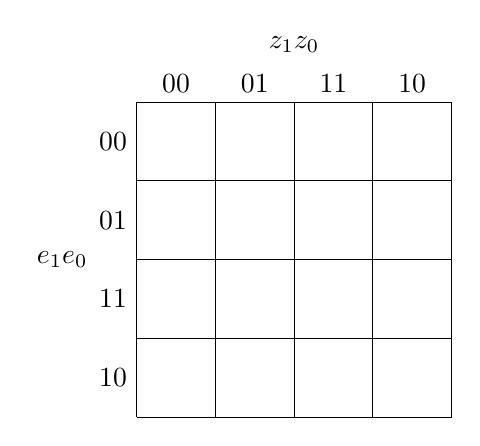
\begin{tikzpicture}[
 pi/.style={fill,draw,circle,minimum size=.1cm},
 pi1/.style={pi,red},
 ]
 \draw (0,0) grid (4,4);
 \draw (2,4) node[above=.5cm] {$z_1z_0$}
 (0,2) node[left=.5cm]  {$e_1e_0$};
 \foreach \p/\code in {0/$00$,1/$01$,2/$11$,3/$10$} {
 	\draw[xshift=.5cm] (\p,4) node[above] {\code};
 	\draw[yshift=3.5cm,yscale=-1] (0,\p) node[left]  {\code};
 }
 
 \draw[shift={(.5,.5)},inner sep=.1mm]
 (0,3) node[]   {$$}
 (0,2) node[]   {$$}
 (0,1) node[]   {$$}
 (0,0) node[]   {$$}
 
 (1,3) node[]   {$$}
 (1,2) node[]   {$$}
 (1,1) node[]   {$$}
 (1,0) node[]   {$$}
 
 (2,3) node[]   {$$}
 (2,2) node[]   {$$}
 (2,1) node[]   {$$}
 (2,0) node[]   {$$}
 
 (3,3) node[]   {$$}
 (3,2) node[]   {$$}
 (3,1) node[]   {$$}
 (3,0) node[]   {$$}
 
 
 ;
 %Beschriftung
 %	\foreach \p/\code in {2/$11$,3/$10$} {
 %		\draw[xshift=.5cm] (\p,4) node[above] {\code};
 %		\draw[yshift=3.5cm,yscale=-1] (0,\p) node[left]  {\code};
 %	}
 
 \end{tikzpicture} 
